\begin{figure*}[ht]
\centering
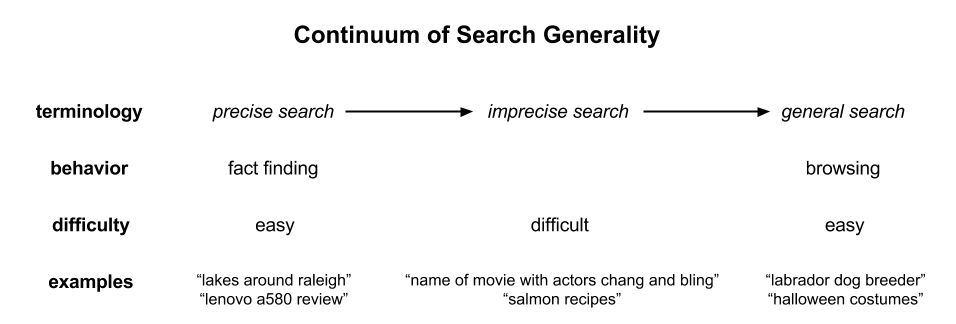
\includegraphics[width=\textwidth]{images/terminologydiagram}
\caption{ Our proposed continuum of search generality characterizes search according to the breadth of the information being sought. We expect that specific and broad information is generally easy for users to describe and find, but that this is not true with information in the ``no man�s land" between.}
\label{fig:searchcontinuum}
\end{figure*}




According to recent reports, mobile search will soon surpass desktop search as measured by both queries and ad revenue \cite{MobileQueries}\cite{MobileRevenue}. Despite this growing importance, Cui and Roto \cite{Cui:2008} and Church and Oliver \cite{Church:2011} find that current mobile search interfaces lead users to seek only information that is fairly specific (e.g. fact-finding) or quite general (e.g. browsing). Both types of information are easy to retrieve with queries, and easy to find in search results.

Ideally mobile users should not have to limit themselves in this way, and indeed often they do not, either because they try and fail to do so, or because of their pressing need for the information. Then their lack of knowledge about the information they seek and the limited query capability of the mobile interface \cite{Kamvar:2009} can force them to repeatedly reformulate their queries, and explore results extensively. For example, a user may seek a specific actor. If she cannot remember the name of the actor (in which case she would directly search by name), she might instead search for an actor who worked with the actor they seek.

As Lee \textit{et al.} \cite{Lee:2012} point out, this ``no man's land" of \textit{imprecise} search (neither very general nor very specific) is more common than we might think, and some search engines have begun offering partial solutions. Search suggestions offer to complete keyword sets automatically in real time, helping users form better queries. Google's Knowledge Graph \cite{GoogleKnowledgeGraph} displays related facts from databases, making results easier to navigate. Yet neither solution is complete.

Our proposed continuum of search generality from precise search to general search is based on the breadth of the information being sought, and is illustrated in Figure \ref{fig:searchcontinuum}.

We believe that we can improve imprecise mobile search further by exploiting the entity-relationship structure in many online information sources to give mobile users a better overview of their results. Such sources might include movies and crew in IMDb~\cite{imdb}, songs and artists in Pandora~\cite{pandora}, and friends in Facebook~\cite{Facebook}. These overviews reduce cognitive load through recognition, allow navigation of search results by attributes rather than only keyword \cite{Hearst:2002}, and guide users in the query reformulations that are typical of imprecise search.

In this paper, we present \textit{GraphTiles}, a visual search interface designed help mobile users perform imprecise and general searches. The interface displays an incomplete portion of the local entity-relationship neighborhood: a thumbnail of the current page alone in the left column, some pages one link away in the middle column, and other pages two links away in the right column. To see the complete neighborhood, users can scroll the central and right columns vertically. While this layout implies many links, it does not indicate exactly where the links are between the second and third columns. Users can reveal these locations by selecting a page thumbnail from these columns, triggering an \textit{interactive reordering} that highlights pages linked to the selection and places them onscreen or nearly so. Users can restore the original (better known) order by deselecting the page.